\documentclass[alg,ngerman,seminar,pdf,article]{unitext}

\usepackage[utf8]{inputenc}

\usepackage{enumitem}
\makeatletter
\let\mdwNote\note                        % make \IEEEproof do same as \proof
\let\note\@undefined                        % undefine \proof
\makeatother

\usepackage{calligra}
\usepackage{amsmath}
\usepackage{amsthm}
\usepackage{stmaryrd}
\usepackage{float}
\usepackage{subfig}
\usepackage{framed}

\usepackage{algorithmic}
\usepackage{algorithm}
\floatname{algorithm}{\algorithmName}
\numberwithin{algorithm}{section}
\algsetup{linenosize=\normalsize, linenodelimiter=.}
\renewcommand{\algorithmicrequire}{\textbf{Eingabe:}}
\renewcommand{\algorithmicensure}{\textbf{Ausgabe:}}

%\usepackage{gnuplottex}

\usepackage{tikz}
\usepackage{environ}
\makeatletter
\newsavebox{\measure@tikzpicture}
\NewEnviron{scaletikzpicturetowidth}[1]{%
  \def\tikz@width{#1}%
  \def\tikzscale{1}\begin{lrbox}{\measure@tikzpicture}%
  \BODY
  \end{lrbox}%
  \pgfmathparse{#1/\wd\measure@tikzpicture}%
  \edef\tikzscale{\pgfmathresult}%
  \BODY
}
\makeatother

%\usepackage[final]{pdfpages}
\usepackage[draft]{pdfpages}

\newtheoremstyle{note} % name
                {10pt} %Space above               
                {10pt} %Space below
                {\itshape} %Body font
                {} %Indent amount
                {\bfseries} % Theorem head font
                {:} %Punctuation after theorem head
                {.5em} %Space after theorem head
                {} %Theorem head spec (can be left empty, meaning ‘normal’)

\newtheoremstyle{definition} % name
                {10pt} %Space above               
                {10pt} %Space below
                {} %Body font
                {} %Indent amount
                {\bfseries} % Theorem head font
                {} %Punctuation after theorem head
                {\newline} %Space after theorem head
                {} %Theorem head spec (can be left empty, meaning ‘normal’)

\newtheoremstyle{theorem} % name
                {10pt} %Space above               
                {10pt} %Space below
                {\itshape} %Body font
                {} %Indent amount
                {\bfseries} % Theorem head font
                {} %Punctuation after theorem head
                {.5em} %Normal Space after theorem head
                {} %Theorem head spec (can be left empty, meaning ‘normal’)

\newtheoremstyle{example} % name
                {10pt} %Space above               
                {10pt} %Space below
                {} %Body font
                {} %Indent amount
                {\bfseries} % Theorem head font
                {} %Punctuation after theorem head
                {\newline} %Space after theorem head
                {} %Theorem head spec (can be left empty, meaning ‘normal’)




\theoremstyle{definition}
%\newtheorem{definition}{Definition}[chapter]
\newtheorem{definition}{Definition}[section]
\newtheorem*{standaloneProof}{\proofName}

\theoremstyle{theorem}
\newtheorem{theorem}[definition]{\theoremName}
\newtheorem{lemma}[definition]{\lemmaName}
\newtheorem{corollary}[definition]{\corollaryName}
\newtheorem{problem}[definition]{\problemName}

\theoremstyle{example}
\newtheorem{example}[definition]{\exampleName}

\theoremstyle{remark}
\newtheorem{remark}[definition]{\remarkName}
\newtheorem{observation}[definition]{\observationName}

\renewcommand{\proofname}{\proofName}

%%% named references
\newcommand{\defRef}[1]{\definitionName \ \ref{def:#1}}
\newcommand{\remRef}[1]{\remarkName \ \ref{rem:#1}}
\newcommand{\theoRef}[1]{\theoremName \ \ref{theo:#1}}
\newcommand{\corRef}[1]{\corollaryName \ \ref{cor:#1}}
\newcommand{\lemRef}[1]{\lemmaName \ \ref{lem:#1}}
\newcommand{\probRef}[1]{\problemName \ \ref{prob:#1}}
\newcommand{\figRef}[1]{\figureName \ \ref{fig:#1}}
\newcommand{\algRef}[1]{\algorithmName \ \ref{alg:#1}}

%%% Highlighting and indexing of terms
\newcommand{\term}[1]{\emph{#1}\index{#1}}

% reduce space around cdot
\let\oldcdot=\cdot
\def\cdot{\negthinspace\oldcdot\negthinspace}

\def\notmid{\!\!\:\!\not|\;}

\newcommand{\N}{\mathbb{N}}
\newcommand{\R}{\mathbb{R}}
\newcommand{\Rd}{\R^d}
\newcommand{\Sd}[1]{\mathbb{S}_{#1}}
\newcommand{\Bd}{\mathbb{B}_{d}}
\newcommand{\I}{[0,1]}
\newcommand{\RdEx}{\widehat{\mathbb{R}}^d}
\newcommand{\REx}{\widehat{\R}}

\newcommand{\ointerv}[1]{\ensuremath{\left]#1\right[}}
\newcommand{\lopen}[1]{\ensuremath{\left]#1\right]}}
\newcommand{\ropen}[1]{\ensuremath{\left[#1\right[}}
\newcommand{\func}[3]{\ensuremath{{#1} \colon {#2} \to {#3}}}

\newcommand{\eps}{\varepsilon}
\newcommand{\timeDom}{\mathcal{T}}
\newcommand{\disjUnion}{\ensuremath{\dot{\cup}}}

\newcommand{\outEdges}{\delta^+}
\newcommand{\inEdges}{\delta^-}

%% Graphs
\newcommand{\graph}{\mathcal{N}}
\newcommand{\A}{A}
\newcommand{\tExp}[1]{\ensuremath{\graph^{#1}}}
\newcommand{\redNetw}[2]{\tExp{#1}\!/{#2}}
\newcommand{\pathSet}{\mathcal{P}}

%% Möbius groups
\DeclareMathOperator{\GM}{GM}
\newcommand{\GMRd}{\GM(\Rd)}
\DeclareMathOperator{\M}{M}
\newcommand{\MRd}{\M(\Rd)}
\newcommand{\MSd}{\M(\Sd{d-1})}

%% Operators %%
\DeclareMathOperator{\grad}{grad}
\DeclareMathOperator{\im}{im}
\DeclareMathOperator{\Conf}{Conf}
\DeclareMathOperator{\head}{head}
\DeclareMathOperator{\tail}{tail}

%% sets of differentiable functions %%
\newcommand{\diffPw}[3]{C^{#1}_{\mathcal{P}}({#2}, {#3})}
\newcommand{\diffRdPw}[2]{\diffPw{#1}{#2}{\Rd}}
\newcommand{\diffRd}[2]{C^{#1}({#2}, \Rd)}
\newcommand{\diff}[3]{C^{#1}({#2}, {#3})}

%% Special functions/operators
\newcommand{\arclength}[1]{\ell({#1}, \mathcal{P})}
\newcommand{\norm}[1]{\left\Vert{#1}\right\Vert}
\newcommand{\inner}[2]{\left\langle{#1},{#2}\right\rangle}

%% Set definitions
\newcommand{\where}{\:|\:} % for set definitions
\newcommand{\setDef}[2]{\left\{{#1} \:|\: {#2}\right\}}


%%%%%%%% textual formatings %%%%%%%%%%
\newcommand{\resp}{\mbox{resp.}\ }
\newcommand{\st}{\mbox{s.t.}\ }

%%%%%%%% text colors %%%%%%%%
\newcommand{\red}[1]{\textcolor{red}{#1}}
\newcommand{\green}[1]{\textcolor{green}{#1}}
\newcommand{\yellow}[1]{\textcolor{yellow}{#1}}
\newcommand{\blue}[1]{\textcolor{blue}{#1}}


\graphicspath{{images/}}

\title{Quickest flows over time}
\author{Henning Basold}
%\date{October 17th, 2011}
%\dozent{Dr. Iris Reinbacher}
\betreuer{Björn Hendriks}

\renewcommand{\purposename}{Purpose}
\renewcommand{\abstractname}{Abstract}

%\keywords{Elliptic Curve Cryptography, Parallelization, Key Agreement}
%\makeglossary
%\makeindex
%\makenomenclature

\begin{document}

\titelblatt             %%% obligatorisch
%\zusammenfassung        %%% obligatorisch, in der Datei abstract.tex
%\cleardoublepage
\tableofcontents        %%% obligatorisch
%\listoftables           %%% optional
%\listoffigures          %%% optional
%\abkuerzung             %%% optional, in der Datei abbreviation.tex

\starttext
%\chapter{Mathematical Foundations}\label{chap:math}

\section{Grundlegende Definitionen und Problembeschreibung}\label{sec:problem}

\subsection{Einleitung}

In diesem Seminar wird ein Verfahren vorgestellt, mit dem allgemeine dynamische
Flussprobleme in Netzwerken approximiert werden können. Ein dynamischer Fluss
besitzt im
Gegensatz zu einem statischen Fluss eine Zeitkomponente. Diese gibt an, wie
lange ein Fluss benötigt, um über eine Kante zu gelangen. Der erste Ansatz
dazu war, dass die Zeit genügend fein zu unterteilen (kleinere Zeitintervalle
als Transportzeiten) und für jeden Zeitschritt die Knoten zu replizieren und
entsprechend den Transportzeiten Kanten einzufügen. Hier können dann die
bekannten Flussalgorithmen verwendet werden. Allerdings führt diese Art
zu sehr großen Netzwerken. Trotzdem werden wir diese Idee weiter verfolgen.
Dabei werden wir eine Approximation angeben, sodass die Größe des Netzwerks
polynomiell in der Zeit sein wird.

Wir werden diese Technik auf das Quickest-Transshipment-Problem anwenden,
das in einem anderen Seminarvortrag vorgestellt wird.

\subsection{Begriffe}
Zunächst soll die verwendete Notation geklärt werden.

\begin{definition}
    Wir verwenden übliche \term{Netzwerke} bzw. gerichtete, endliche \term{Graphen}
    $\graph = (V, \A)$ bestehend aus Knoten und Kanten,
    wobei $n := |V|$ und $m := |\A|$.
    
    Einem solchen Netzwerk werden einige Funktionen zugeordnet:
    \begin{itemize}
        \item $\head : \A \rightarrow V$, $(u,v) \mapsto v$
        \item $\tail : \A \rightarrow V$, $(u,v) \mapsto u$
        \item $\outEdges : V \rightarrow 2^\A$,
            $v \mapsto \setDef{e \in \A}{tail(e) = v}$
        \item $\inEdges : V \rightarrow 2^\A$,
            $v \mapsto \setDef{e \in \A}{head(e) = v}$
    \end{itemize}
    
    Der Graph wird mit Funktionen angereichert, die mit als Eingabe
    für die Probleme dienen.
    \begin{itemize}
        \item $\tau : \A \rightarrow \R$, $e \mapsto \tau_e$ -- \term{Laufzeit}
        \item $u : \A \rightarrow \R$, $e \mapsto u_e$ -- \term{Kapazität}
        \item $c : \A \rightarrow \R$, $e \mapsto c_e$
            -- \term{Kosten} pro Flusseinheit
    \end{itemize}
\end{definition}

Zur Einführung werden wir zuerst den \term{statischen Fluss} definieren, dieser
hat im Gegensatz zum dynamischen keine Zeitkomponente.

\begin{definition}
    Sei $S \subseteq V$ die Menge der \term{Terminale} mit $S = S^+ \;\dot{\cup}\; S^-$
    und Funktionen
    \begin{itemize}
        \item $D : S^+ \rightarrow \R_+$ -- \term{Zulauf}
        \item $D : S^- \rightarrow \R_-$ -- \term{Bedarf}
    \end{itemize}
    die $\sum_{v \in S} D(v) = 0$ erfüllen. Wir nehmen dabei an, dass keine Kanten in
    Quellen hineinführen und keine aus Senken heraus: $\inEdges(S^+) = \emptyset$ und
    $\outEdges(S^-) = \emptyset$.
    
    Wenn $S^+ = \{s\}$ und $S^- = \{t\}$, dann schreiben wir kurz $d = D(s) = -D(t)$.
\end{definition}

\begin{remark}
    Um die Betrachtungen zu vereinfachen, wollen wir die Terminalknoten
    für jede Ware durch jeweils einen Knoten ersetzen. Dazu können
    Knoten $\setDef{s_i}{i \in K}$ und $\setDef{t_i}{i \in K}$ zu dem
    Netzwerk hinzugefügt werden. Diese werden mit den jeweiligen
    Terminalknoten verbunden: $(s_i, v)$ für alle $v \in S_i^+$ und
    $(v,t_i)$ für alle $v \in S_i^-$. Diesen Knoten wird die Kapazität $\infty$
    und Laufzeit $0$ zugeordnet. Diese Knoten werden zu den neuen Terminalen
    erklärt.

    Dann lassen sich die Bedarfsfunktionen pro Ware definieren:
    $D(i) = \sum_{v \in S_i^+} D(vi)$.

    Wir werden also lediglich Netzwerke betrachten, die pro Ware nur eine
    Quelle und Senke haben.

    % BjH: Diese Bemerkung bezieht sich auf mehrere Waren, was aber erst weiter unten eingeführt wird (insbesondere auch die Symbole mit den $i$-Indizes).
\end{remark}

\begin{definition}[Statischer Fluss mit einer Ware]
    Ein statischer Fluss ist eine Abbildung $x : \A \rightarrow \R_+$ mit
    \[ \sum_{e \in \outEdges(v)} x(e) - \sum_{e \in \inEdges(v)} x(e) = 0
        \quad, \text{alle } v \in V \setminus S. \]

    Ein solcher Fluss sollte im Allgemeinen folgende Eigenschaften erfüllen:
    \begin{itemize}
        \item Erfüllung von Bedarf und Zulauf:
            \[ \sum_{e \in \outEdges(v)} x(e) - \sum_{e \in \inEdges(v)} x(e) = D(v)
                \quad, \text{alle } v \in S. \]
        \item Zulässigkeit:
            \[ x(e) \leq u(e) \quad, \text{alle } e \in \A \]
    \end{itemize}

    Einem Fluss können außerdem die nötigen Kosten zugeordnet werden:
        \[ c(x) = \sum_{e \in \A} c(e) \cdot x(e). \]
\end{definition}

\begin{definition}[Mehrere Waren]
    Die oben definierten Flüsse können lediglich einen Bedarf erfüllen, will
    man unterschiedliche Waren zulassen, geht man zu sogenannten
    \term{Multicommodity}-Problemen über.

    Dazu wird eine Menge von Waren $K = \{1, \ldots, k\}$ sowie die jeweiligen
    Terminale $S_i = S_i^+ \disjUnion S_i^- \subseteq V$ festgelegt. Für diese
    Terminale muss dann jeweils der Bedarf angegeben werden:
    \begin{enumerate}
        \item $\func{D_i}{S_i^+}{\R_+}$ -- Zulauf
        \item $\func{D_i}{S_i^-}{\R_-}$ -- Bedarf
    \end{enumerate}

    Wir setzen $S := \bigcup\limits_{i \in K} S_i$.
\end{definition}

\begin{definition}[Statischer Fluss mit mehreren Waren]
    Die Waren induzieren eine Familie von statischen Flüssen
    $x = \{\func{x_i}{\A}{\R_+}\}_{i \in K}$. Dabei ist $x$ zulässig, wenn die
    Kapazität durch den Transport aller Waren nicht verletzt wird:
    \begin{align*}
        & \sum_{i \in K} x_i(e) \leq u(e) \quad \text{, alle } e \in \A.
    \end{align*}

    Die Kosten werden entsprechend auch über alle Waren aufsummiert,
    wobei die Kosten auch hier durch eine Familie von Funktionen
    $\{\func{c_i}{\A}{\R_+}\}_{i \in K}$ bestimmt werden.
    \begin{align*}
        & c(x) = \sum_{e \in A} \sum_{i \in K} c_i(e) \cdot x_i(e)
    \end{align*}
\end{definition}

Nachdem wir nun statische Flüsse ohne Zeitkomponente kennengelernt haben,
wollen wir Flüsse über Zeit (dynamische Flüsse) betrachten. Werden direkt
die allgemeinere Definition mit mehreren Waren geben.
% BjH: Im letzten Satz fehlt ein Wort.

\begin{definition}
    Ein \term{dynamischer Fluss} ist eine Familie von Funktionen
    $\{\func{f_i}{\A \times \ropen{0,T}}{\R_+}\}_{i \in K}$.
    $f_i(e,t)$ ist die \term{Flussrate}, die zur Zeit $t$ an der Kante $e$ anliegt.
    Dabei muss \\ $\lim_{t \to T} f_i(e,t) = 0$ gelten. Dann kann $f$ stetig
    auf $\ropen{T, +\infty}$ fortgesetzt werden.
    % BjH: Wo kommt das $\lim_{t \to T}$ her? Zumindest kann ich es im Paper nicht finden. Ein Limes setzt Konvergenz voraus; darf die Flussrate nicht pl\"otzlich auf Null gehen? (siehe auch lim unten.)

    Schreibe auch: $\func{f_i(e)}{\ropen{0,T}}{\R_+}$ mit $f_i(e)(t) = f_i(e,t)$.

    Um das Verhalten eines Flusses zu analysieren, definieren wir uns die Last an
    einem Knoten durch
    \[
        F_i(v, t) =
            \int_0^t \left(
                \sum_{e \in \outEdges(v)} f_i(e, \theta) -
                \sum_{e \in \inEdges(v)} f_i(e, \theta - \tau(e)) \right) \;d\theta .
    \]

    Der Fluss muss dann folgendes erfüllen:
    \begin{itemize}
        \item $F_i(v, t) \leq 0$ für alle $v \in S_i^-$ (Senken)
            und $t \in \ropen{0,T}$
        \item $F_i(v, t) = 0$ für alle $v \in V \setminus S$ und $t \in \ropen{0,T}$
            ohne Speicher bzw. $F_i(v, t) \leq 0$ wenn Speicher zugelassen ist.
            Dann muss aber auch $\lim_{t \to T} F_i(v, t) = 0$,
            damit kein Fluss zurückbleibt.
    \end{itemize}

    %Der Gesamtfluss auf einer Kante ist die Summe über alle Warenflüsse:
    %\[
    %    f(e, t) := \sum_{i \in K} f_i(e,t)
    %\]

    Ein dynamischer Fluss wird \term{zulässig} genannt, wenn der Gesamtfluss
    die Kapazität nicht übersteigt:
    \[
        \sum_{i \in K} f_i(e,t) \leq u(e) \quad \text{, alle } e \in \A
                                                \text{ und } t \in \ropen{0,T}.
    \]

    Auch einem dynamischen Fluss werden wieder Kosten zugeordnet:
    \[
        c(f) = \sum_{i \in K} \sum_{e \in \A} c_i(e) \int_0^T f_i(e,t) \: dt.
    \]
\end{definition}

\begin{remark}
    Der Fluss $f_i(e,t)$ kommt zur Zeit $t + \tau(e)$ bei $head(e)$ an. Daher folgt
    sofort, dass $f_i(e,t) = 0$, wenn $t \in \ropen{T - \tau(e), T}$.
\end{remark}

Nun wollen wir uns dem \term{Flusswert} zuwenden. Dieser ist insofern wichtig,
als dass er angibt, ob der Bedarf für eine Ware erfüllt ist.

\begin{definition}
    Seien $x$ ein statischer und $f$ ein dynamischer Fluss. Der \term{Flusswert}
    ist dann jeweils definiert durch

    \[
        |x| = \sum_{i \in K} \sum_{v \in S_i^+} \sum_{e \in \inEdges(v)} x_i(e)
    \]
    und
    \[
        |f| = \sum_{i \in K} \sum_{v \in S_i^+}
                \sum_{e \in \inEdges(v)} \int_0^T f_i(e,t) \: dt
            = \sum_{i \in K} \sum_{v \in S_i^+} F_i(v,T).
    \]
    Die zweite Gleichung gilt dabei, da ein Fluss eine Senke nicht wieder
    verlässt und Summe und Integral dann vertauscht werden dürfen.
\end{definition}

Das letzte Werkzeug, das wir benötigen werden, sind \term{Pfadzerlegungen}
von Flüssen.

\begin{definition}\label{def:path_flow}
    Seien $x$ ein statischer und $f$ ein dynamischer Fluss.
    Sei weiterhin $\pathSet$ eine endliche Menge von Pfaden von $S_i^+$ nach
    $S_i^-$. Wenn es eine Familie $\{\func{x_i}{\pathSet}{\R_+}\}_{i \in K}$
    bzw. $\{\func{f_i}{\pathSet \times \ropen{0,T}}{\R_+}\}_{i \in K}$ gibt,
    dann ist $\pathSet$ eine \term{Pfadzerlegung}, wenn gilt
    \[
        x_i(e) = \sum_{P \in \pathSet : e \in P} x(P) \quad \text{, für alle } e \in \A
    \]
    bzw.
    \[
        f_i(e, t) = \sum_{P \in \pathSet : e \in P} f(P, t - \tau(P \downarrow e)) .
    \]
    Dabei ist $P \downarrow e$ die Einschränkung von $P$ auf die Kanten \emph{vor} $e$
    und $\tau(P) = \sum_{e \in P} \tau(e)$ die natürliche Erweiterung von $\tau$ auf
    Pfade.

    Wenn Speicher zugelassen ist, müssen Verzögerungen bei dynamischen Flüssen
    mit einbezogen werden.
\end{definition}


\section{Zeiterweiterte Netzwerke}

Unser Ziel ist ein polynomielles Approximationsschema für Quickest-Flow-Probleme.
Die Idee dabei ist, ein Netzwerk $\graph$ in ein \term{zeiterweitertes Netzwerk}
umzuwandeln. Dazu werden für jeden Zeitschritt Kopien der Knoten von $\graph$
angelegt. Dabei gibt die Zeitkomponente den Zeitpunkt eines Flusses an. Daher
werden in dem neuen Graph zwei Knoten genau dann verbunden, wenn die Knoten
im ursprünglichen Graphen durch eine Kante $e \in \A$ verbunden gewesen sind und
sie $\tau(e)$ Zeitschritte entfernt sind. Zusätzlich werden sogenannte
\term{Haltekanten} eingefügt. Diese verbinden jeweils die Kopie eines
Terminals mit der Kopie vom nächsten Zeitschritt. Diese Stellen den Speicher
für bisher nicht verschickte bzw. bereits angekommene Waren dar.
Daher wird dann auch eine Kopie einer Quelle bei Zeit $0$ zur neuen Quelle
und eine Kopie einer Senke bei Zeit $T-1$ zur neuen Senke erklärt.

Wir nehmen dabei an, dass die Zeiten ganzzahlig sind. Dies ist durch Skalierung
der Zeit auf die gewünschte Genauigkeit für Anwendungen problemlos möglich.

\begin{definition}[Zeiterweitertes Netzwerk]
    Sei $(\graph, \tau)$ ein Netzwerk mit Waren $K$. Seien außerdem
    $\tau(e) \in \N$ für alle $e \in \A$ und $T \in \N$.

    Setze $\timeDom := \{0, 1, \ldots, T-1\}$. Wir definieren damit das
    \term{zeiterweiterte Netzwerk} $\tExp{T} = (V^T, \A^T)$ durch
    \begin{itemize}
        \item $V^T = V \times \timeDom$ (schreibe $v_t = (v, t)$ und
            $V_t = \{v_t \in V^T\}$)
        \item $\A^T = \setDef{e_t = (v_t, u_{t + \tau(e)})}
                        {e = (v, u) \in \A \text{ und } t, t + \tau(e) \in \timeDom}
                    \cup H$ \\
            mit „\term{holdover arcs}“ bzw. \term{Speicherkanten} \\
            $H = \setDef{(v_t, v_{t+1})}
                        {v \in S_i \text{ und } t, t + 1 \in \timeDom}$
        \item $\func{u^T}{\A^T}{\REx = \R \cup \{\infty\}}$ mit
                $u^T(e_t) = \begin{cases}
                    u(e)    &, e_t \not\in H \\
                    \infty  &, e_t \in H
                \end{cases}$
        \item $\func{c^T}{\A^T}{\R}$ mit
                $c^T(e_t) = \begin{cases}
                    c(e)    &, e_t \not\in H \\
                    0       &, e_t \in H
                \end{cases}$
        \item $S_i^{+,T} = \setDef{v_0 \in V^T}{v \in S_i^+}$, \\
                $S_i^{-,T} = \setDef{v_{T-1} \in V^T}{v \in S_i^-}$ und damit \\
                $S_i^T = S_i^{+,T} \disjUnion S_i^{-,T} \text{ für alle } i \in K$
    \end{itemize}
    Sollte Speicher an Knoten $V \setminus S$ zugelassen sein, dann müssen analog
    zu $H$ weitere Speicherkanten eingefügt werden.
\end{definition}

\begin{remark}
    Da in Netzwerken $\inEdges(s) = \emptyset$ für alle $s \in S_i^+$ und
    $\outEdges(t) = \emptyset$ für alle $t \in S_i^-$ (d.h. Quellen und Senken
    können keine inneren Knoten auf Flüssen sein), kann in der obigen Definition
    auch $\REx$ durch $\R$ ersetzt werden, wenn man die Kapazität der
    Speicherkanten $(v_t, v_{t+1}) \in H$ größer oder gleich $|D_i(v)|$ für
    $v \in S_i$ wählt. Wenn der Fluss diesen Bedarf übersteigen darf,
    muss die Kapazität entsprechend größer gewählt werden.
\end{remark}

\begin{example}
    Wir wollen uns ein einfaches Beispiel für ein zeiterweitertes Netzwerk 
    ansehen. Dazu sehen wir uns \figRef{ex_time_expanded_1} an. In dem
    Netzwerk deklarieren wir nur $s$ als Quelle und $t$ als Senke:
    $S^+ = \{s\}, S^- = \{t\}$.

    \begin{figure}[H]
    \centering
    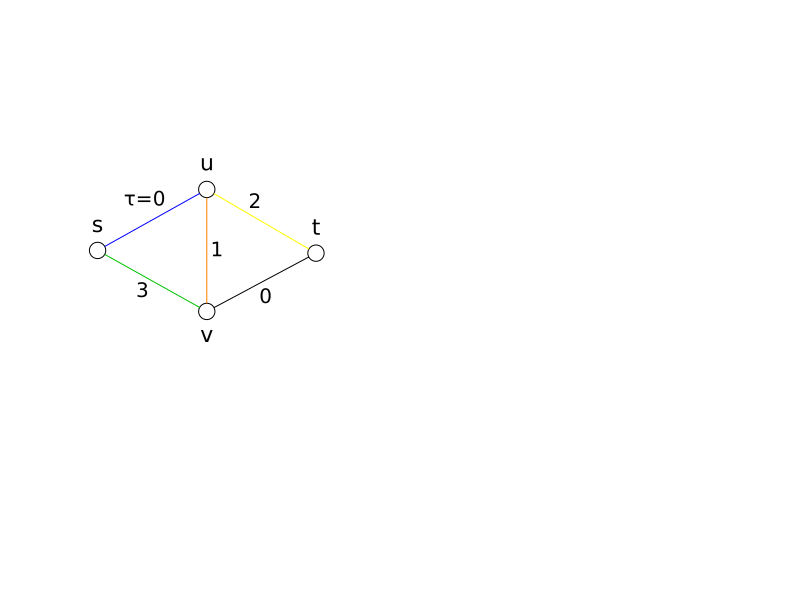
\includegraphics[width=0.5\textwidth]{ex_time_expanded_1}
    \caption{Einfaches Netzwerk, mit eingefärbten Kanten, sodass diese im
                zeiterweiterten wiedererkannt werden können}
    \label{fig:ex_time_expanded_1}
    \end{figure}

    Wir betrachten $T = 6$ und damit $\timeDom = \{0, \ldots, 5\}$. An den
    Kanten sind die Zeiten $\tau$ notiert. Wir nehmen außerdem an, dass
    an dem Knoten $u$ Speicher zugelassen ist. Dann ergibt sich
    des Netzwerk $\tExp{T}$ in \figRef{ex_time_expanded_2}.

    \begin{figure}[H]
    \centering
    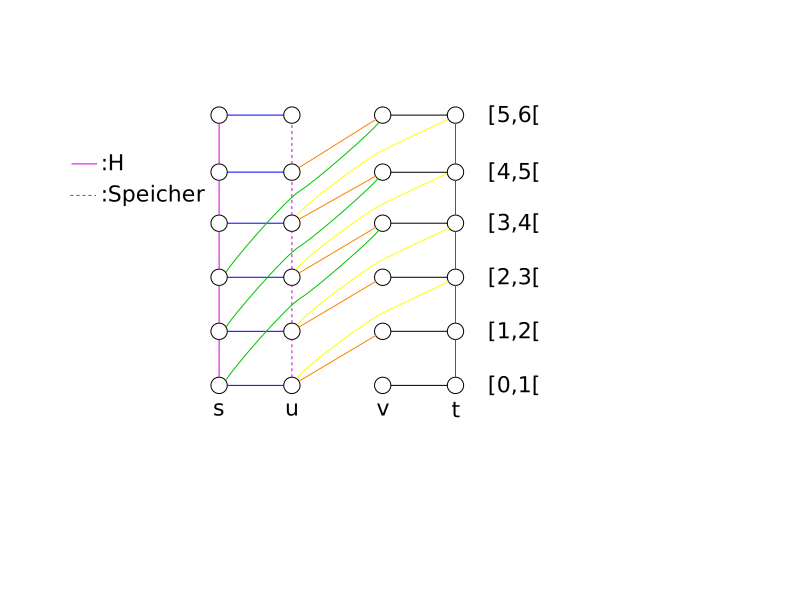
\includegraphics[width=0.7\textwidth]{ex_time_expanded_2}
    \caption{Beispiel für ein zeiterweitertes Netzwerk}
    \label{fig:ex_time_expanded_2}
    \end{figure}
\end{example}

Da wir dynamische Flüsse mit Hilfe von Algorithmen für statische Flüsse
konstruieren wollen, müssen wir zwischen Flüssen $f$ in $\graph$ und
Flüssen $x$ in $\tExp{T}$ wechseln können:

\begin{lemma}\label{lem:static_dyn_conv}
    Ein statischer Fluss $\func{x_i}{\A^T}{\R_+}$ in $\tExp{T}$ entspricht einem
    dynamischen Fluss $\func{f_i}{\A \times \ropen{0,T}}{\R_+}$ in $\graph$
    mit gleichem Flusswert und Kosten und umgekehrt. Dabei gilt:
    \begin{enumerate}
        \item $f_i(e,t) := x_i(e_{\lfloor t \rfloor})$ und
        \item $x_i(e_t) := \int_t^{t+1} f_i(e, \theta) \: d\theta$
    \end{enumerate}
\end{lemma}

Dieser Sachverhalt ist zwar sehr einfach, hat allerdings das Problem, dass das
Netzwerk $\tExp{T}$ sehr groß wird. Denn $|V^T| = |V| \cdot |\timeDom| = n \cdot T$.
Da aber $T$ in der Größe $\log T$ kodiert wird, hängt $V^T$ nicht mehr polynomiell
von der Eingabe ab.

Die Idee ist nun, das Netzwerk $\tExp{T}$ wieder zu verkleinern, so dass es
eine polynomielle Größe erreicht, indem unnötige Zeitschritte entfernt werden.
Das führt zu den \term{skalierten Netzwerken}:

\begin{definition}\label{def:red_network}
    Sei $(\graph, \tau)$ Netzwerk und $0 < \Delta$, so dass $T/\Delta \in \N$
    und $\tau(e)/\Delta \in \N$ für alle $e \in \A$. Wir setzen
    $\tau' := \tau/\Delta$ und damit
    $\redNetw{T}{\Delta} := \tExp{T/\Delta}$ für $(\graph, \tau')$.
    
    Ein Knoten $v_t$ entspricht dann einem Zeitverlauf im Intervall
    $\ropen{t \Delta, (t+1) \Delta}$. Daher müssen die Kosten und Kapazitäten
    auf $c' := c \cdot \Delta$ und $u' := u \cdot \Delta$ korrigiert werden.
\end{definition}

\begin{lemma}\label{lem:reduced_static_dyn_conv}
    Sei $0 < \Delta$ und $(\graph, \tau)$ wie oben. Dann entspricht ein statischer
    Fluss $x_i$ in $\redNetw{T}{\Delta}$ einem Fluss
    $\func{f_i}{\A \times \ropen{0, T}}{\R_+}$ in $\graph$ mit gleichen Kosten
    und umgekehrt.
    
    \begin{proof}
        Wende \lemRef{static_dyn_conv} auf $x_i$ an, dies ergibt einen Fluss
        $\func{\hat{f}_i}{\A \times \ropen{0, T/\Delta}}{\R_+}$. Mit Skalierung der
        Zeit um $\Delta$ ergibt sich $f$. Die Kosten ändern sich dabei nicht.
    \end{proof}
\end{lemma}

Wenn $p(\Delta) \in O(T)$ mit einem Polynom $p$ gewählt werden kann, funktioniert
dieses Verfahren gut, da dann $T/\Delta \in O(T)$. Leider wird dies in den meisten
Fällen nicht möglich sein.
Die Idee ist nun, $\Delta$ so zu wählen, dass man $\tau(e)$ „vernünftig“ zum
nächsten Vielfachen von $\Delta$ runden kann. Damit könnte man
\lemRef{reduced_static_dyn_conv} anwenden. Allerdings kann ein solches
Runden zu Problemen führen. Diese sollen in den nächsten beiden Beispielen
veranschaulicht und daraus Bedingungen an $\Delta$ gestellt werden.

\begin{example}
    Sei $(\graph, \tau)$ mit einem Teil wie in \figRef{ex_inc_time_1} gegeben.
    Die Kapazitäten seien dabei überall $1$. Außerdem sind in der Abbildung die
    beiden möglichen Pfade über die Kante $e_3$ dargestellt.

    \newsavebox{\tempbox}
    \begin{figure}[H]
    \sbox{\tempbox}{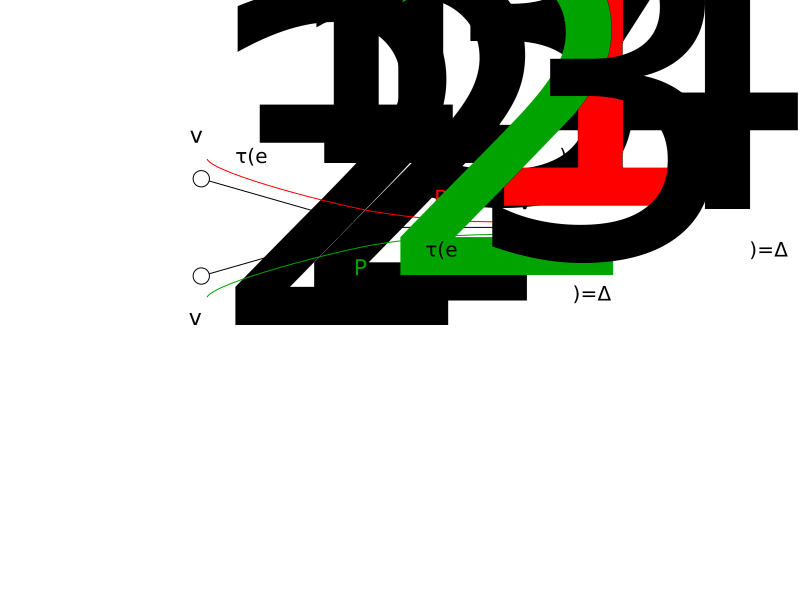
\includegraphics[width=0.5\textwidth]{ex_inc_time_1}}
    \subfloat{\usebox{\tempbox}}%
    \qquad
    \subfloat{\vbox to \ht\tempbox{%
      \vfil
        \begin{tabular}{ l| c c c c c }
          t (in $\Delta/2$) & 0 & 1 & 2 & 3 & 4 \\ \hline
          f($e_1$)          & \red{1} & 0 & 0 & 0 & 0 \\
          f($e_2$)          & \green{1} & 0 & 0 & 0 & 0 \\
          f($e_3$)          & 0 & \red{1} & \green{1} & 0 & 0 \\
          L($e_3$)          & 0 & 1 & 2 & 1 & 0
        \end{tabular}
      \vfil}}%
      \caption{Netzwerk, in dem sich ein maximaler Fluss beim Aufrunden staut;
        dazu ein Verlauf dieses maximalen Flusses}\label{fig:ex_inc_time_1}
    \end{figure}

    Die Tabelle in \figRef{ex_inc_time_1} gibt den Zeitverlauf eines maximalen Flusses
    $f$ an. $L$ ist dabei die Last auf einer Kante (der Fluss, der sich
    derzeit auf der Kante befindet).

    Wie man sieht, befinden sich zum Zeitpunkt $2$ zwei Flusseinheiten gleichzeitig
    auf $e_3$. Werden nun die Zeiten zu $\Delta$ aufgerundet, ergibt sich der
    Netzwerkausschnitt aus \figRef{ex_inc_time_2}.

    \begin{figure}[H]
    \centering
    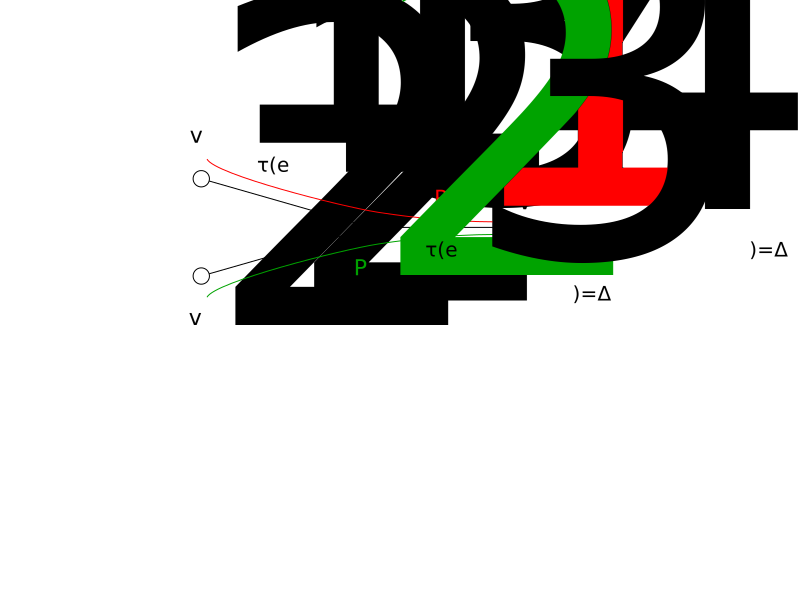
\includegraphics[width=0.5\textwidth]{ex_inc_time_2}
    \caption{Beispiel für ein Netzwerk mit gerundeten Zeiten}
    \label{fig:ex_inc_time_2}
    \end{figure}

     Überträgt man den Fluss $x$ nun
    in dieses Netzwerk, muss $x$ auf $e_1$ oder $e_2$ verzögert werden, da $P_1$
    und $P_2$ an dieser Stelle nicht gleichzeitig benutzt werden können.
    Auf $e_3$ „staut“ sich der Fluss.

    Insgesamt benötigt der Fluss dann $2\Delta$ statt lediglich $\frac{3}{2}\Delta$
    Zeiteinheiten.
\end{example}

Daraus ergibt sich die erste Bedingung, die an $(\graph, \tau)$ gestellt wird. Wir
bezeichnen dabei mit $T^*$ die jeweils optimale Laufzeit.
\begin{framed}
\begin{enumerate}[label={(A\arabic*)}]
    \item Die optimale Laufzeit $\widetilde{T}^*$ eines Flussproblems in
        $(\graph, \widetilde{\tau})$ approximiert die optimale Laufzeit $T^*$
        desselben Problems in $(\graph, \tau)$,
        d.h. $|\widetilde{T}^* - T^*| \leq \eps$,
        wenn $|\widetilde{\tau}(e) - \tau(e)| \leq \eps$. \label{a1}
        % BjH: Hier ist mir noch nicht ganz klar. Entlang eines Pfades k\"onnten sich doch die Rundungen \"uber verschiedene Kanten aufsummieren.
        % HB: tatsächlich verschiebt man den ganzen Fluss überall nur um \eps und damit
        %       insgesamt auch nur um \eps (sonst würde Lemma 3.4 auch nicht funktionieren)
\end{enumerate}
\end{framed}

\begin{example}

    Wir betrachten nun ein Netzwerk, in dem die Situation genau umgekehrt ist:
    im Netzwerk mit aufgerundeten Zeiten lässt sich ein viel besserer Fluss
    konstruieren, als im Originalnetzwerk. Wir betrachten dazu das Netzwerk
    in \figRef{ex_val_red_1}. Dort verlaufen alle Pfade $s-t$ über die
    Kante $e$. Wenn nun die Laufzeiten zu $\Delta$ aufgerundet werden,
    ergibt sich das Netzwerk in \figRef{ex_val_red_2}.

    \begin{figure}[H]
    \centering
    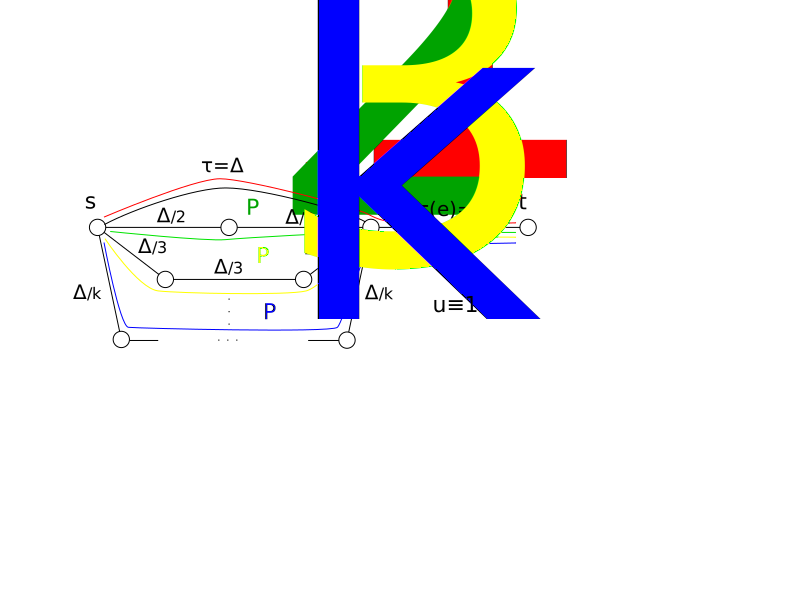
\includegraphics[width=0.6\textwidth]{ex_val_red_1}
    \caption{Awesome Image}
    \label{fig:ex_val_red_1}
    \end{figure}
    
    Man sieht, dass wenn man einen Fluss $f$ auf allen Kanten gleichzeitig losschickt,
    dieser versetzt am Knoten $v$ ankommt. Siehe dazu auch
    $f(e)$ in der Tabelle. Soll dieser Fluss wieder im Originalnetzwerk
    interpretiert werden, muss fast der komplette Fluss verworfen werden, denn
    sonst wäre $f(e) = k > 1 = u(e)$, wenn $k > 1$.
    
    % \newsavebox{\tempbox}
    \begin{figure}[H]
    \sbox{\tempbox}{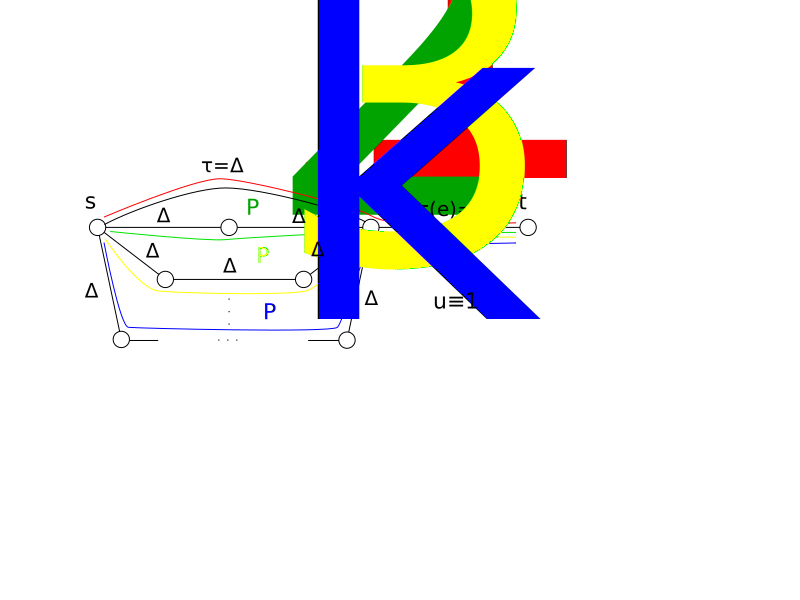
\includegraphics[width=0.5\textwidth]{ex_val_red_2}}
    \subfloat{\usebox{\tempbox}}%
    \qquad
    \subfloat{\vbox to \ht\tempbox{%
      \vfil
        \begin{tabular}{ l| c c c c c c c }
          t (in $\Delta/2$) & 0 & 1 & 2 & 3 & \ldots & k & \ldots \\ \hline
          f($P_1$)  & \red{1} & 0 & 0 & 0 & \ldots & \red{1} & \\
          f($P_2$)  & \green{1} & 0 & 0 & 0 & \ldots & \green{1} & \\
          f($P_3$)  & \yellow{1} & 0 & 0 & 0 & \ldots & \yellow{1} & \\
          \vdots    & \vdots & & & & & \vdots & \ldots \\
          f($P_k$)  & \blue{1} & 0 & 0 & 0 & \ldots & \blue{1} & \\
          f($e$)    & 0 & \red{1} & \green{1} & \yellow{1} & \ldots & \blue{1} &
        \end{tabular}
      \vfil}}%
      \caption{Netzwerk $(\graph, \tau')$, in dem nach Aufrunden ein viel größerer
        Fluss möglich ist}\label{fig:ex_val_red_2}
    \end{figure}    
\end{example}

Aus diesem Beispiel ergibt sich die zweite Bedingung:
\begin{framed}
\begin{enumerate}[start=2, label={(A\arabic*)}]
    \item Eine Lösung $\widetilde{f}$ in $(\graph, \widetilde{\tau})$ muss
        ohne großen Verlust in einen Fluss $f$ in $(\graph, \tau)$
        umgewandelt werden können: $||\widetilde{f}| - |f|| \leq \eps$.
        \label{a2}
\end{enumerate}
\end{framed}

Diese beiden Eigenschaften sind auch hinreichend für eine beliebig genaue
Approximation:
\begin{corollary}
    Sei $\graph$ ein Netzwerk mit zwei Laufzeiten $\tau_1$ und $\tau_2$, so dass
    \ref{a1} und \ref{a2} erfüllt sind.
    Dann kann ein optimaler Fluss $f_1^*$ in $(\graph, \tau_2)$ approximiert werden,
    wenn ein optimaler Fluss $f_2^*$ in $(\graph, \tau_2)$ approximiert werden kann.
    % BjH: Wo ist $\tau_1$ geblieben?
    % HB: das ist schon so gemeint: ich kann f_1^* in (N, tau_2) approximieren.
    %       Das wollen wir ja gerade: Zeiten runden (tau_2) und dann für
    %       das ursprüngliche Netzwerk approximieren.

    \begin{proof}    
        Sei $\eps > 0$ und o.B.d.A. $\tau_2 - \tau_1 \leq \eps$ und seien
        $f_1^*$ und $f_2^*$ jeweils optimale Flüsse, die bei
        $T_1^*$ bzw. $T_2^*$ enden. Nach \ref{a1} ist $T_2^* - T_1^*\leq \eps$.

        Sei $f_2$ eine Approximation von $f_2^*$ in $(\graph, \tau_2)$ mit
        $||f_2| - |f_2^*|| \leq \eps$ und Ende $T_2 - T_2^* \leq \eps$.

        Dann kann $f_2$ als ein Fluss $f_1$ in $(\graph, \tau_1)$
        mit Ende $T_1$ interpretiert werden. Es gilt nach \ref{a2}:
        \begin{align*}
            ||f_1| - |f_1^*|| & \leq ||f_1| - |f_2^*| + \eps| \\
                            & \leq ||f_2| + \eps - |f_2^*| + \eps| \\
                            & \leq ||f_2| - |f_2^*|| + 2 \eps \\
                            & \leq 3 \eps
            % BjH: Sollte Epsilon hier nicht immer au\ss{}erhalb des Betrags stehen? Wenn die Differenz innerhalb des Betrags negativ ist, kann das Epsilon den Absolutwert verkleinern.
            % HB: Ich habe hier nur ersetzt, was in (A1) steht : |f_1^*| \leq |f_2^*| - \eps
        \end{align*}
        und
        \begin{align*}
            T_1 - T_1^*  & \leq T_2 + \eps - T_2^* + \eps \\
                & \leq \eps + 2\eps \\
                & = 3 \eps
            % BjH: Hier und oben fehlen vermutlich die Betr\"age.
            % HB: habs oben hinzugeschrieben: Annahme ist, dass tau_2 nach oben aufrundet.
        \end{align*}
        
        Somit kann $f_1^*$ in $(\graph, \tau_2)$ beliebig genau approximiert werden.
    \end{proof}
\end{corollary}

%\begin{observation}
%    TODO: Beobachtung 5, zur Realisierung von \ref{a1} und \ref{a2} mit Speicher.
%\end{observation}



\section{Gleichförmig reduzierte zeit-expandierte Netzwerke}\label{sec:unif_cond}

TODO: Definiere Fluss auf Pfaden!

\subsection{Quickest Transshipment mit einer Ware (singlecommodity)}

Zu QTP:
\begin{theorem}\label{theo:qtp_flow_ex}
    Sei $T \geq T^*$. Setze $\Delta := \frac{\eps^2 T}{n}$ und
    $T' := \lceil (1+\eps)^3 T / \Delta \rceil \Delta$.
    Dann gilt:
    \begin{enumerate}
        \item in $\redNetw{T'}{\Delta}$ existiert ein statischer Fluss $x$ mit
            Bedarf $|x| = (1 + \eps)D$ und Kosten $c(x) \leq (1+\eps)C$.
        \item aus $x$ kann ein dynamischer Fluss $f$ in $\graph$ berechnet werden,
            der bei $(1+\eps)T'$ endet und für den $|f| = D$ und $c(f) \leq C$
            gilt.
    \end{enumerate}
\end{theorem}

Bevor wir diesen Satz beweisen, folgern wir daraus den Algorithmus:

TODO:
\begin{theorem}
    QTP-FPTAS-Core
\end{theorem}

TODO: Einbettung in Suchframework

\begin{theorem}\label{theo:slow_flow}
    Sei $\func{f(e)}{\ropen{0, T + \delta}}{\R_+}$ ein dynamischer Fluss in $(\graph, \tau)$
    mit $|f| = D$ und $c(f) \leq C$ und einer endlichen Zerlegung in Flüsse $f(P)$
    auf Pfaden $P \in \pathSet$. Sei $\eps > 0$ und $(\graph, \tau')$ das
    gleiche Netzwerk mit geänderten Zeiten, für die
    $\left|\tau(e) - \tau'(e)\right| \leq \frac{\eps^2T}{n}$ gilt. Definiere
    einen Fluss in $(\graph, \tau')$
    \[
    \tilde{f}(P)(t) := \frac{1}{1+\eps} \frac{1}{\eps T}
                            \int_{t - \eps T}^{t} f(P)(\theta) \; d\theta \text{ .}
    \]
    Dann gilt für $\tilde{f}$:
    \begin{enumerate}
        \item $\tilde{f}$ endet bei $\delta + T + \eps T + \eps^2 T$
        \item $\tilde{f}$ verläuft nur auf Pfaden aus $\pathSet$
        \item $|\tilde{f}| = \frac{D}{1 + \eps}$
        \item $c(\tilde{f}) \leq \frac{C}{1 + \eps}$
    \end{enumerate}
    
    \begin{proof}
        TODO: in Tex und Anpassung an $T + \delta$.
    \end{proof}
\end{theorem}

\begin{lemma}\label{lem:relaxed_flow}
    Sei $\func{f^*(e)}{\ropen{0,T^*}}{\R_+}$ ein dynamischer Fluss in $(\graph, \tau)$
    mit Bedarf $|f^*| = D$ und Kosten $c(f^*) \leq C$. Für alle $\delta \geq 1$ und
    und $T \geq T^*$ existiert ein dynamischer Fluss
    $\func{f(e)}{\ropen{0, \delta T}}{\R_+}$ mit $|f| = \delta D$ und
    $c(f) \leq \delta C$. Dabei ist $f$ kreisfrei/kommt ohne Speicher aus, wenn $f^*$
    dies ist/tut.
    
    \begin{proof}
        TODO: in Tex
    \end{proof}
\end{lemma}

Zu QTP:
\begin{theorem}\label{theo:qtp_opt_flow}
    TODO: Existenz optimaler Fluss mit Pfadzerlegung und ohne Speicher
     (Corollary 4.5).
\end{theorem}

\begin{standaloneProof}[\theoRef{qtp_flow_ex}a]
    Nach \theoRef{qtp_opt_flow} existiert ein optimaler Fluss $f^*$, der
    keinen Speicher benötigt und nur auf Pfaden verläuft.
    Setze $\delta = (1 + \eps)^2$ und wende \lemRef{relaxed_flow} mit
    $T \geq T^*$ an und erhalte einen Fluss $f$ der bei $(1 + \eps)^2 T$ endet.
    $f$ besitzt damit eine endliche Pfadzerlegung, hat Bedarf
    $|f| = (1 + \eps)^2 D$ und Kosten $c(f) \leq (1 + \eps)^2 C$.
    
    Setze nun $\tau'(e) := \lceil \tau(e) / \Delta \rceil \Delta$ für
    alle $e \in \A$. Dann ist offensichtlich
    $|\tau(e) - \tau'(e)| \leq \Delta = \frac{\eps^2 T}{n}$.
    Da $\delta T = T + 2 \eps T + \eps^2 T$ ist, liefert
    \theoRef{slow_flow} uns einen Fluss $\tilde{f}$ in $(\graph, \tau')$
    der bei
    \begin{align*}
        & T + 2 \eps T + \eps^2 T + \eps T + \eps^2 T \\
        & = T + 3 \eps T + 2 \eps^2 T \\
        & \leq T + 3 \eps T + 3 \eps^2 T + \eps^3 T \\
        & = (1 + \eps)^3 T \leq T'
    \end{align*}
    endet. $\tilde{f}$ hat Bedarf
    $|\tilde{f}| = \frac{|f|}{1+\eps} = (1 + \eps) D$ und ebenso
    Kosten $c(\tilde{f}) \leq (1 + \eps) C$.
    
    Da $\tau'$ und $T'$ nach Konstruktion ganzzahlig durch
    $\Delta$ teilbar sind, lässt sich $\tilde{f}$ als statischer Fluss $x$ in
    $\redNetw{T'}{\Delta}$ interpretieren, der die gewünschten
    Eigenschaften hat.
    
    \begin{flushright}\qed \end{flushright}
\end{standaloneProof}

\begin{lemma}\label{lem:path_decomp}
    Eine Pfadzerlegung $\pathSet$ von einem statischen Fluss $x$ in
    $\redNetw{T'}{\Delta}$ kann in eine Pfadzerlegung $\pathSet'$ des
    zugehörigen dynamischen Flusses $f'$ in $(\graph, \tau')$ 
    transformiert werden. Dabei wird $\ropen{0, T'}$ in $T'/\Delta$
    disjunkte Teilintervalle zerlegt, auf den $f'(P)$ auf allen $P \in \pathSet'$
    konstant ist.
    
    \begin{proof}
        TODO: in Tex
    \end{proof}
\end{lemma}

\begin{standaloneProof}[\theoRef{qtp_flow_ex}b]
    Der Fluss $x$ in $\redNetw{T'}{\Delta}$ induziert einen Fluss $f'$ in
    $(\graph, \tau')$:
    \begin{align*}
        & \func{f'(e)}{\ropen{0,T'}}{\R_+} \\
        & f'(e)(t) = x(e)(\lfloor t \rfloor) \\
        & \quad \text{ (d.h. } f'(e)(\theta) = x(e)(t)
            \text{ für alle } \theta \in \ropen{t, t+1} \text{ ) }
    \end{align*}
    Offensichtlich ist $f'$ ein zulässiger Fluss in $(\graph, \tau')$ und
    hat die gleichen Eigenschaften wie $x$ (Bedarf $(1+\eps)D$, Kosten $(1+\eps)C$).
    
    Mit \lemRef{path_decomp} bekommen wir eine Pfadzerlegung $\pathSet'$.
    Der erste Teil von \theoRef{slow_flow} liefert uns wieder einen Fluss
    $f$ auf $\ropen{0, (1 + \eps)T'}$ mit Bedarf $D$ und Kosten
    $c(f) \leq C$.
    
    TODO: evtl. \theoRef{slow_flow} aufteilen.
    
    \begin{flushright}\qed \end{flushright}
\end{standaloneProof}

TODO: Laufzeitanalyse

\begin{remark}
    Alles was wir für den Beweis von \theoRef{qtp_flow_ex} benutzt haben, ist
    unabhängig von einem speziellen Flussproblem gültig
    (bis auf \theoRef{qtp_opt_flow}). Dies liefert uns also ein „Framework“
    zur Konstruktion von Algorithmen und entsprechenden Beweisen.
\end{remark}

\subsection*{Quickest Transshipment mit mehren Waren (multicommodity)}
Dies wollen wir direkt ausnutzen, um ein das obige Verfahren auf mehrere
Waren zu verallgemeinern. Die Approximation hiervon ohne Speicher ist allerdings
NP-hart (TODO: Quelle [19] dazu betrachten), da eine optimale Lösung ohne Speicher
Zyklen enthalten kann. Mit Speicher kann allerdings einfach gewartet werden,
anstatt einen Zyklus zu benutzen.

Allerdings kann aus einem Pfad, auf dem Speicher verwendet wird, nicht mehr wie
in dem Beweis von \theoRef{slow_flow} der Fluss auf Kanten rekonstruiert werden.
Das kommt daher, dass dort erwartet wird, das sich die Laufzeit eines Flusses
direkt aus $\tau$ ergibt. Mit Speicher ist dies aber nicht der Fall
(s. dazu Definition von $\tau(P \downarrow e)$).

TODO: definiere $P^\delta$ und $\tau(P^\delta \downarrow e)$, lasse dabei $\delta$
eine Funktion $V \to \R_+$ sein.

TODO: verallgemeinere \theoRef{slow_flow}, um Speicher mit dieser Definition zuzulassen
und setze in den Beweisen im letzten Abschnitt $\delta = 0$

Dann folgt dies alles als Korollar.


\section{Nicht gleichförmig reduzierte zeit-expandierte Netzwerke}\label{sec:nonunif_cond}
Die gleichmäßige Unterteilung der Zeit durch $\timeDom = \{0,1, \ldots, T-1\}$ kann bei
anderen Problemen zu schlechten Ergebnissen führen. Wir wollen dazu kurz das Problem
des „Earliest Arrival Flows“ und dazu ein kritisches Beispiel betrachten.

TODO: Problem

TODO: Beispiel + Bild

Man kann dieses Problem umgehen, indem man den Zeitverlauf anders unterteilt. In dem
Beispiel würde die Unterteilung in Intervalle der Größe $\frac{1}{2}$
genügen ($\timeDom = \{0, \frac{1}{2}, 1\}$). Wir wollen uns für diesen Fall nur
die entsprechende Definition des zeitertweiterten Netzwerks ansehen.

\begin{definition}[zeiterweitertes Netzwerk mit beliebigen Zeitintervallen]
    Sei $(\graph, \tau)$ und $L = (\theta_q)_{q \in R}$, wobei $R = \{0, \ldots, r\}$,
    sodass
    \[
        0 = \theta_0 < \theta_1 < \ldots < \theta_r < T.
    \]
    Setze $\theta_{r+1} = T$.
    Dann ist das \term{L-zeitexpandierte Netzwerk} $\tExp{L} = (V^L, \A^L)$
    gegeben durch
    \begin{itemize}
        \item $V^L = V \times R$ (schreibe $v_q = (v, q)$ und
            $V_q = \{v_q \in V^L\}$)
        \item $\A^L = \setDef{e_q = (v_q, u_{m(e, q)})}
                        {e = (v, u) \in \A, q \in R, \theta_q + \tau(e) \leq \theta_r}
                    \cup H$, \\
            \text{ wobei } $H = \setDef{(v_q, v_{q+1})}
                                    {v \in S_i \text{ und } q, q+1 \in R}$
    \end{itemize}

    Dabei ist $\func{m}{\A \times R}{R}$ definiert durch
    \[
        m(e, q) := \min \setDef{q' \in R}{\theta_q + \tau(e) \leq \theta_{q'}}.
    \]
    $m$ bestimmt also das Intervall, zwischen welchen die Kante $e$ transportiert.
    Die Rest ist analog wie bei den ursprünglichen zeiterweiterten Netzwerken
    definiert.
\end{definition}

\begin{remark}
    Offensichtlich ergibt sich mit einer Unterteilung $L = (0, 1, \ldots, T-1)$
    wieder $\tExp{T} = \tExp{L}$. Also sind L-zeiterweiterte Netzwerke
    eine Verallgemeinerung.
\end{remark}

TODO: wie werden diese benutzt?

%%%% Einträge im Glossar werden durch den Befehl
%%%    \glossar{begriff}{erklärung}
%%% vorgenommen.

\glossar{Gruppe}{Eine \emph{Gruppe} ist eine
Menge mit einer zweistelligen assoziativen Verknüpfung mit Einselement
und inversen Elementen.}

\glossar{Abelsche Gruppe}{Eine Gruppe
heißt \emph{abelsch}, wenn die Verknüpfung kommutativ ist.}

\glossar{Ä}{ein Eintrag, der mit einem Umlaut beginnt.}


\nocite{*}
\bibliography{lit}
%\printglossary
%\printindex
\anhang

\end{document}
